\chapter{TINJAUAN PUSTAKA}
\label{chap:tinjauanpustaka}

\section{Penelitian Terkait}
\label{sec:penelitianterkait}

Terdapat 5 penelitian terkait yang menjadi dasar dari penelitian ini
yang dapat dilihat pada gambar \ref{fig:fishbone}.
% Contoh input gambar
\begin{figure}[H]
  \centering

  % Ubah dengan nama file gambar dan ukuran yang akan digunakan
  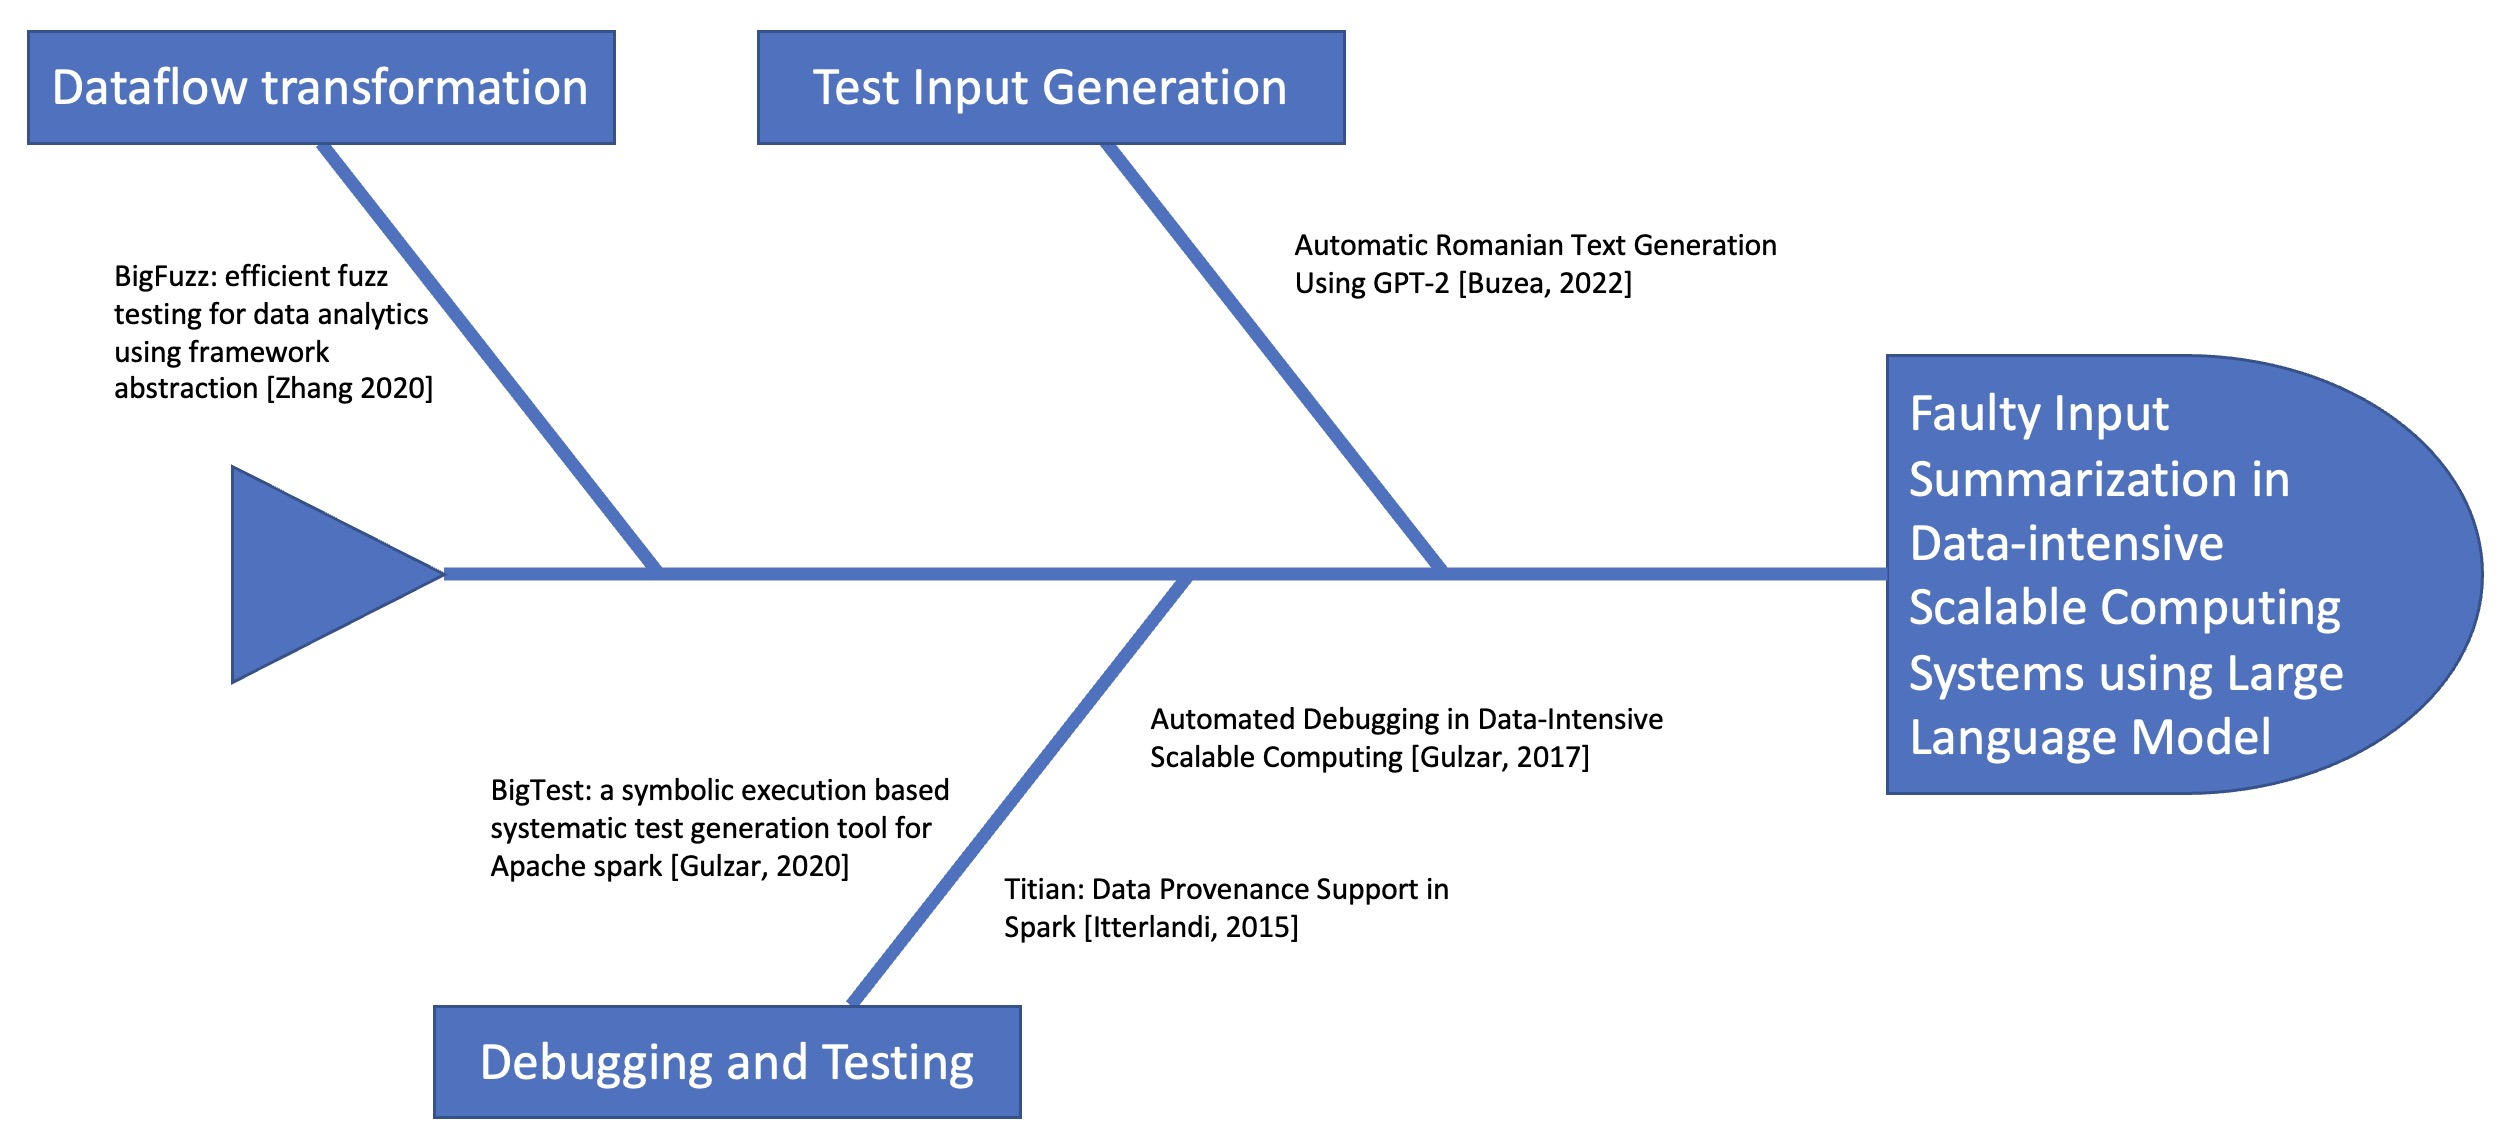
\includegraphics[scale=0.18]{gambar/StateOfTheArt.jpg}

  % Ubah dengan keterangan gambar yang diinginkan
  \caption{Diagram \emph{Fishbone}}
  \label{fig:fishbone}
\end{figure}

% \begin{table}[H]
%   \centering
%   \caption{Penelitian Terkait}
%   \begin{tabular}{|c|c|c|c|c|}
%     \hline
%     Sitasi & Data & Metode & \emph{Library} & Pengujian \\
%     % get value from penjelasan di bawah
%     \hline
%     \cite{gulzar2017} & 
%     \hline
%     \cite{zhang2021} 
%     \hline
%     \cite{gulzar2020} 
%     \hline
%     \cite{interlandi2015} 
%     \hline
%     \cite{buzea2022} 
%     \hline
%   \end{tabular}
  
%   \label{tab:penelitianterkait}
% \end{table}

Adapun penjelasan tentang penelitian terkait yang menjadi 
dasar dari penelitian ini adalah sebagai berikut:
\begin{enumerate}
\item \emph{Automated Debugging in Data-Intensive Scalable Computing}

Penelitian yang dilakukan oleh Muhammad Ali Gulzar dan rekan-rekannya fokus pada pengembangan beban kerja \emph{Big Data Analytics}. Mereka menghadapi tantangan dalam \emph{debugging}, terutama terkait dengan data tidak terstruktur dan asumsi yang salah mengenai data, yang sering menyebabkan kesalahan dalam program. Untuk mengatasi masalah ini, penelitian ini memperkenalkan metode baru yang disebut BIGSIFT, yang berfokus pada menemukan lokasi data yang menyebabkan kegagalan. Metode yang digunakan yaitu menggabungkan isolasi kesalahan otomatis dalam rekayasa perangkat lunak dengan \emph{provenans} data dalam sistem basis data. Hasil dari penelitian ini adalah peningkatan drastis dalam akurasi dalam menentukan lokasi kesalahan, dengan hasil yang lebih akurat hingga ribuan hingga jutaan kali lipat dibandingkan dengan metode sebelumnya seperti provenans data Titian dan \emph{Delta Debugging}. Dengan demikian, penelitian ini berpotensi memberikan manfaat besar dalam mempercepat proses \emph{debugging} pada beban kerja \emph{Big Data Analytics}, sehingga pengembang dapat mengidentifikasi dan memperbaiki masalah lebih efisien~(\cite{gulzar2017}).

\item \emph{BigFuzz: Efficient Fuzz Testing for Data Analytics Using Framework Abstraction}

Dalam penelitian yang dilakukan oleh Qian Zhang dan timnya, mereka mengatasi tantangan dalam pengujian otomatis untuk sistem data-intensive scalable computing (DISC), yang sangat penting untuk menangani kumpulan data besar dalam konteks analisis big data. Masalah utamanya terletak pada kompleksitas intrinsik dari aplikasi berbasis data semacam itu, di mana data seringkali tidak lengkap, terus berubah, dan sulit untuk diprediksi. Pengujian \emph{fuzzing} tradisional, meskipun efektif di domain lain seperti keamanan, menghadapi hambatan yang signifikan ketika diterapkan langsung pada analisis big data. Alasannya termasuk lamanya latensi sistem DISC, tidak praktisnya cakupan cabang konvensional, dan kesulitan dalam menghasilkan data yang bermakna dengan mutasi acak. Untuk mengatasi tantangan ini, para peneliti mengusulkan alat pengujian \emph{fuzzing} yang dipandu cakupan yang baru untuk analisis big data, yang disebut BigFuzz. Alat ini berfokus pada pengujian logika aplikasi daripada peningkatan cakupan kode kerangka kerja, dengan mengabstraksi kerangka kerja DISC menggunakan spesifikasi. BigFuzz juga menggunakan operator \emph{schema-aware data mutation} berdasarkan analisis mendalam tentang jenis kesalahan aplikasi DISC. Hasil penelitian menunjukkan bahwa BigFuzz secara signifikan mempercepat proses \emph{fuzzing}, meningkatkan cakupan kode, dan meningkatkan deteksi kesalahan dalam aplikasi DISC, menjadikannya alat berharga untuk \emph{debugging} beban kerja analisis \emph{big data}, dapat diterapkan pada beragam program, dan mampu menemukan lebih banyak kesalahan dibandingkan dengan pendekatan terkini yang menggunakan eksekusi simbolik~(\cite{zhang2021}).

\item \emph{BigTest: A Symbolic Execution Based Systematic Test Generation Tool for Apache Spark}

Muhammad Ali Gulzar dan timnya melakukan penelitian dalam bidang sistem komputasi berbasis data yang besar (DISC), seperti MapReduce milik Google, Apache Hadoop, dan Apache Spark, yang digunakan luas dalam layanan produksi. Meskipun aplikasi DISC sangat populer, seringkali kualitas aplikasinya kurang baik karena kurangnya pengujian yang menyeluruh dan otomatis. Saat ini, pengujian aplikasi DISC biasanya hanya menggunakan contoh kecil acak dari data masukan, yang mungkin tidak cukup untuk menemukan masalah dalam program. Pengujian aplikasi DISC memiliki tantangan tersendiri karena menggabungkan operasi aliran data dan relasional, serta fungsi yang bisa sangat kompleks.Untuk mengatasi masalah ini, para peneliti memperkenalkan kerangka pengujian putih yang baru bernama BigTest. BigTest digunakan untuk program Apache Spark dan secara otomatis menghasilkan data buatan untuk pengujian yang efektif dan efisien. BigTest menggabungkan eksekusi simbolik fungsi pengguna dengan spesifikasi logis operasi aliran data dan relasional untuk mengeksplorasi semua jalur dalam aplikasi DISC. Hasil eksperimen menunjukkan bahwa BigTest mampu menemukan dua kali lipat lebih banyak masalah daripada menggunakan seluruh dataset dengan waktu pengujian yang jauh lebih singkat (194 kali lebih cepat). BigTest diimplementasikan sebagai alat baris perintah berbasis Java dengan file biner pra-kompilasi. Pengguna dapat menyesuaikan preferensi melalui file konfigurasi, termasuk program target, batasan eksplorasi \emph{loop}, dan pemilihan penyelesaian teorema. Penelitian ini berpotensi meningkatkan pengujian aplikasi DISC, sehingga masalah dalam program dapat ditemukan dengan lebih efektif dan efisien~(\cite{gulzar2020}).
\\
\\
\\

\item \emph{Titian: Data Provenance Support in Spark}

Matteo Itterlandi dan timnya mengatasi tantangan yang sulit dalam melakukan \emph{debugging} pada logika pemrosesan data di dalam sistem Data-Intensive Scalable Computing (DISC). Biasanya, \emph{debugging} dalam sistem ini memakan banyak waktu dan usaha karena kurangnya alat \emph{debugging} yang memadai, seringkali memerlukan pengumpulan bukti secara manual dari file log dan mencoba-coba. Untuk mempermudah proses ini, mereka mengembangkan Titian, sebuah perpustakaan yang memungkinkan pelacakan asal data - mengikuti jejak data melalui berbagai transformasi di Apache Spark. Dengan menggunakan ekstensi Spark Titian, ilmuwan data dapat dengan cepat mengidentifikasi data masukan yang menjadi penyebab potensial kesalahan atau hasil yang tidak biasa. Titian terintegrasi dengan baik ke dalam \emph{platform} Spark dan menyediakan dukungan asal data dengan kecepatan interaktif, jauh lebih cepat dibandingkan dengan solusi yang sudah ada, dengan dampak minimal pada kinerja pekerjaan Spark. \emph{Overhead} untuk mengambil jejak data biasanya tidak lebih dari 30\% dari waktu eksekusi pekerjaan dasar. Penelitian ini secara signifikan meningkatkan efisiensi dalam \emph{debugging} logika pemrosesan data dalam sistem DISC, memberikan pendekatan yang lebih efektif dan menghemat waktu bagi ilmuwan data dalam mengidentifikasi dan memecahkan masalah~(\cite{interlandi2015}).

\item \emph{Automatic Romanian Text Generation Using GPT-2}

Marius Cristian Buzea dan timnya melakukan penelitian di bidang pemrosesan bahasa alami (NLP), khususnya dalam menghasilkan teks. Mereka menggunakan model transformer besar yang sudah dilatih sebelumnya seperti GPT-2 dan GPT-3 dari OpenAI, serta BERT dari Google. Penelitian ini mengembangkan model NLG berbasis arsitektur GPT-2 untuk menghasilkan teks dalam bahasa Rumania dengan menggunakan teks yang dianotasi secara manual. Model kecil GPT-2 Rumania, bernama MCBGPT-2, dilatih dan diuji dengan 24 ribu berita. Selain itu, model GPT-2 Rumania yang ada, RoGPT-2, juga digunakan dalam eksperimen. Evaluasi menggunakan metrik otomatis seperti BLEU, ROUGE, BLEURT, dan BERTScore menunjukkan bahwa model MCBGPT-2 dan RoGPT-2 memiliki kinerja yang serupa dalam tugas penghasil teks untuk bahasa Rumania, dengan MCBGPT-2 memerlukan lebih sedikit data untuk proses pelatihannya. Hasil eksperimen menunjukkan bahwa MCBGPT-2 dan RoGPT-2 memberikan kinerja yang hampir sama dalam menghasilkan teks dalam bahasa Rumania, namun MCBGPT-2 memerlukan lebih sedikit data selama pelatihan. Selain itu, arsitektur transformer yang digunakan oleh GPT-2 memungkinkan kecepatan pelatihan yang lebih tinggi dan kemampuan paralelisasi yang lebih baik. Penelitian ini menyimpulkan bahwa model MCBGPT-2 adalah alternatif yang efisien untuk model RoGPT-2 yang ada, terutama dalam menghasilkan kalimat panjang menggunakan data pelatihan yang lebih sedikit~(\cite{buzea2022}).


\end{enumerate}

\section{Dasar Teori}
\label{sec:dasarTeori}

Berikut adalah dasar teori yang digunakan dalam penelitian ini:
% - Sistem DISC
% - Apache Spark
% - Spark Titian
% - Natural Language Processing
% - HuggingFace
% - DistilGPT2
% - FastAPI
% - uvicorn
% - AWS EC2

\subsection{Sistem \emph{Data-Intensive Scalable Computing (DISC)}}

\emph{Data-Intensive Scalable Computing} (DISC) adalah pendekatan
komputasi yang terfokus pada pengolahan dan analisis data dalam
skala besar di mana tujuan utamanya adalah memastikan bahwa data
ini dapat digunakan untuk mendapatkan wawasan berharga, men-dukung
pengambilan keputusan, dan mengidentifikasi pola yang relevan
dalam data tersebut~(\cite{dantas2020}). Hingga saat ini, telah
banyak platform yang dibangun untuk dapat memonitoring proses
kerja sistem DISC~(\cite{dragan2019}). 

Arsitektur DISC menawarkan keuntungan signifikan dalam hal efisiensi dan skalabilitas pemrosesan data. Platform seperti Apache Hadoop dan Apache Spark dirancang untuk memproses data dalam jumlah besar dengan memanfaatkan paralelisme dan distribusi. Dengan pendekatan ini, pemrosesan data menjadi lebih cepat dan biaya operasional dapat dikurangi karena pemrosesan dilakukan secara bersamaan di beberapa node dalam sebuah klaster~(\cite{dean2008}).
Hal ini dapat dilihat pada gambar \ref{fig:DISCArchitecture}.

\begin{figure}[H]
  \centering
  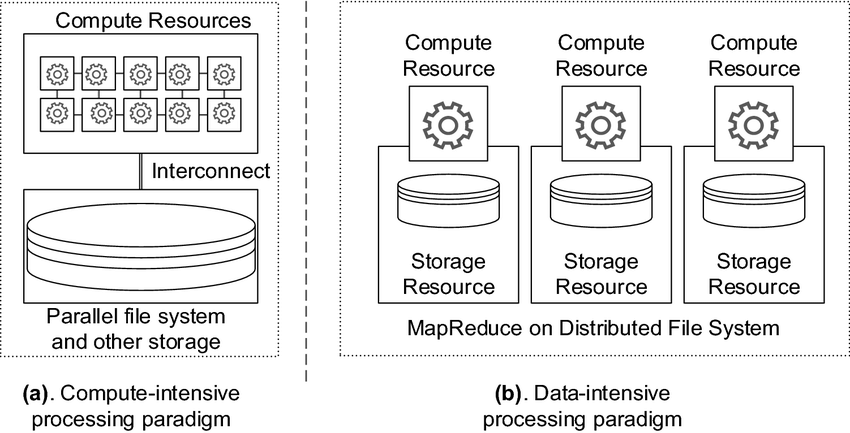
\includegraphics[scale=0.5]{gambar/DISCArchitecture.png}
  \caption{Arsitektur DISC}
  \label{fig:DISCArchitecture}
\end{figure}

Namun, DISC tidak tanpa tantangan. Masalah terkait skalabilitas, keandalan, dan keamanan data seringkali menjadi perhatian utama. Pengelolaan data dalam skala besar memerlukan strategi khusus untuk menjaga integritas data dan melindungi data dari ancaman keamanan yang mungkin muncul. Ini memerlukan upaya tambahan untuk memastikan data aman dan dapat diakses dengan baik~(\cite{hadoop2017}).

Dalam dunia industri, DISC diterapkan secara luas untuk berbagai aplikasi, seperti analisis perilaku pelanggan, deteksi penipuan, dan pengelolaan rantai pasokan. Sebagai contoh, perusahaan e-commerce menggunakan teknik DISC untuk menganalisis data transaksi secara real-time, yang memungkinkan mereka melakukan penentuan harga dinamis dan personalisasi penawaran kepada pelanggan~(\cite{chen2018}).

Teknologi DISC terus berkembang seiring dengan penemuan dan adopsi teknik-teknik baru. Integrasi teknologi pembelajaran mesin dengan platform DISC memungkinkan analisis yang lebih mendalam dan prediktif. Inovasi ini mempercepat proses analisis dan meningkatkan akurasi hasil yang diperoleh, menjadikannya alat yang semakin kuat untuk pengambilan keputusan berbasis data~(\cite{xu2020}).

Untuk memastikan efektivitas dan efisiensi dalam sistem DISC, sejumlah standar dan praktik terbaik telah dikembangkan. Ini mencakup standar untuk format data, pengelolaan metadata, dan strategi backup. Implementasi praktik-praktik ini penting untuk mengurangi kesalahan dan memastikan bahwa data dapat diakses dan digunakan dengan cara yang optimal~(\cite{rodriguez2019}).

Masa depan DISC tampaknya menjanjikan dengan adanya inovasi berkelanjutan dalam komputasi awan dan teknologi big data. Perkembangan seperti komputasi kuantum dan edge computing diharapkan akan lebih meningkatkan kemampuan DISC dalam menangani data dalam skala yang lebih besar dan lebih kompleks. Inovasi ini akan membuka peluang baru untuk analisis data yang lebih canggih dan efisien~(\cite{biau2023}).


\subsection{Apache Spark}

Apache Spark adalah platform pemrosesan data open source yang
sangat kuat dan populer. Dirancang untuk mengatasi tantangan
pemrosesan data dalam skala besar, Spark menyediakan kerangka
kerja yang efisien untuk mengelola dan menganalisis data dalam
volume besar dengan kecepatan tinggi. Salah satu fitur utama
dari Spark adalah kemampuannya untuk menggabungkan pemrosesan
batch dan pemrosesan aliran data dalam satu framework yang
kuat, yang memungkinkan pengguna untuk melakukan analisis data
real-time dan batch dengan efisiensi tinggi. Spark juga mendukung
pemrosesan data terdistribusi dan pemrosesan paralel, yang
membuatnya sangat cocok untuk tugas-tugas yang membutuhkan
komputasi tingkat tinggi. Ini memiliki antarmuka pemrograman
yang beragam, termasuk Python, Scala, dan Java, sehingga dapat
diakses oleh berbagai pengembang. Spark juga memiliki perpustakaan
yang kaya, seperti MLib untuk pembelajaran mesin, SQL untuk kueri
data, dan Streaming untuk pemrosesan aliran data~(\cite{spark}).
Platform ini telah menjadi pilihan populer dalam berbagai
industri, termasuk analisis data, ilmu data, dan pemrosesan
aliran data~(\cite{shaikh2019}).

Apache Spark menawarkan arsitektur yang sangat skalabel yang memudahkan pengolahan data besar dalam lingkungan yang terdistribusi. Arsitektur ini terdiri dari driver, executor, dan cluster manager, yang bekerja sama untuk memproses data dalam skala besar secara efisien. Driver bertanggung jawab untuk mengelola pekerjaan dan membagi tugas ke berbagai executor, yang kemudian melakukan pemrosesan data di node-node dalam cluster. Struktur ini memungkinkan Spark untuk mendistribusikan beban kerja secara merata dan mengelola sumber daya dengan efektif, 
seperti yang digambarkan pada gambar \ref{fig:sparkArsitektur}~(\cite{spark}).

\begin{figure}[H]
  \centering
  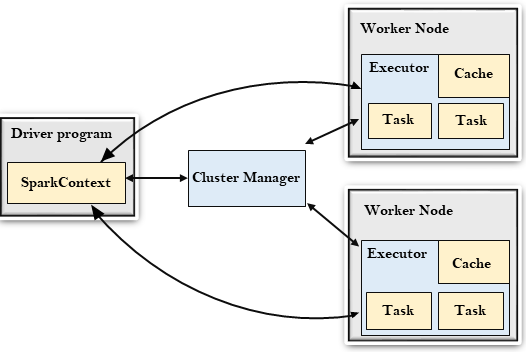
\includegraphics[scale=0.5]{gambar/sparkArsitektur.png}
  \caption{Arsitektur Spark}
  \label{fig:sparkArsitektur}
\end{figure}

Selain itu, Spark menyediakan mekanisme toleransi kesalahan yang kuat, seperti penyimpanan data secara otomatis ke dalam Resilient Distributed Datasets (RDD). RDD adalah struktur data yang memungkinkan pemrosesan data terdistribusi dengan ketahanan terhadap kegagalan. Jika terjadi kegagalan pada node tertentu, Spark dapat memulihkan data yang hilang dari salinan yang ada, sehingga memastikan integritas dan keberlanjutan pemrosesan data. Fitur ini meningkatkan keandalan Spark dalam menghadapi masalah jaringan dan perangkat keras~(\cite{zhang2020}).

Dalam hal performa, Spark unggul dibandingkan dengan teknologi pemrosesan data tradisional seperti Hadoop MapReduce. Spark menggunakan memori sebagai media penyimpanan utama untuk data sementara selama proses pemrosesan, yang secara signifikan meningkatkan kecepatan eksekusi dibandingkan dengan sistem berbasis disk. Ini memungkinkan Spark untuk melakukan analisis yang lebih cepat dan efisien, yang sangat penting dalam aplikasi yang memerlukan pemrosesan data secara real-t
ime~(\cite{zhang2021}).

Penggunaan Apache Spark semakin meluas di berbagai bidang industri, termasuk sektor finansial, kesehatan, dan teknologi. Banyak organisasi memanfaatkan Spark untuk menganalisis data besar guna mendapatkan wawasan yang mendalam dan mendukung keputusan strategis. Dengan dukungan untuk berbagai jenis data dan integrasi yang mudah dengan teknologi big data lainnya, Spark telah menjadi alat yang esensial untuk pemrosesan data yang canggih dan analisis berbasis data besar~(\cite{sharma2022}).

\subsection{Spark Titian}

Spark Titian merupakan sebuah perpustakaan yang dirancang untuk
memungkinkan provenans data interaktif dalam lingkungan Apache Spark.
Titian terintegrasi dengan antarmuka pemrograman Spark, yang
berdasarkan abstraksi \emph{Resilient Distributed Dataset} (RDD)
yang menentukan serangkaian transformasi dan tindakan untuk
memproses kumpulan data. RDD adalah kumpulan data yang terdistribusi
yang dapat dihitung ulang jika terjadi kegagalan.
Data yang dihasilkan dari serangkaian
transformasi tertentu yang menghasilkan RDD dapat disimpan dalam
memori. Spark menjaga sejarah transformasi program sehingga dapat
memulihkan partisi RDD yang hilang dalam
kasus kegagalan. Titian memperkaya abstraksi RDD
dengan kemampuan provenans data yang sangat terinci. Ini
memungkinkan seorang pemrogram Spark untuk mengakses referensi
LineageRDD dari RDD tertentu, memfasilitasi fungsionalitas
pelacakan data, yaitu kemampuan untuk berpindah mundur
(atau maju) dalam aliran data program Spark. Dari referensi
LineageRDD tertentu, yang sesuai dengan posisi dalam eksekusi
program, dapat memanggil transformasi RDD asli apa pun,
menghasilkan RDD baru yang memproses subset data yang
dirujuk oleh LineageRDD. Kemampuan ini menyederhanakan
kemampuan untuk melacak baik ke belakang maupun ke depan
dalam aliran data, memungkinkan eksekusi serangkaian transformasi
RDD asli baru pada data yang dirujuk. Dukungan pelacakan yang
disediakan oleh LineageRDD terintegrasi dengan operator batch
internal Spark dan mekanisme toleransi kesalahan. Akibatnya,
Titian dapat digunakan dalam sesi terminal Spark, menyediakan
dukungan provenans data interaktif bersama dengan kueri ad-hoc
Spark asli~(\cite{interlandi2015}).

\subsection{\emph{Natural Language Processing} (NLP)}

\emph{Natural Language Processing} (NLP) adalah cabang dari kecerdasan buatan yang berfokus pada interaksi antara komputer dan bahasa manusia. Tujuan utama dari NLP adalah untuk memungkinkan komputer untuk memahami, memproses, dan menghasilkan bahasa manusia secara alami~(\cite{jurafsky2021}). NLP telah menjadi bidang penelitian yang sangat penting dalam beberapa tahun terakhir, dengan banyak aplikasi yang berkembang pesat, seperti \emph{chatbots}, \emph{machine translation}, \emph{sentiment analysis}, dan banyak lagi~(\cite{manning2014}). Salah satu alat yang paling populer dalam NLP adalah model bahasa berbasis transformer, seperti GPT-2 dan GPT-3 dari OpenAI, dan BERT dari Google~(\cite{devlin2019}).

Teknologi NLP telah mengalami kemajuan pesat dengan diperkenalkannya model-model transformer yang canggih. Model seperti GPT-3 menggunakan arsitektur yang sangat besar dengan miliaran parameter, memungkinkan mereka untuk menghasilkan teks yang sangat mirip dengan bahasa manusia. Kemampuan ini telah membuka kemungkinan baru dalam aplikasi seperti penulisan otomatis, penjawaban pertanyaan, dan pembuatan konten yang lebih kontekstual dan relevan. Arsitektur dasar dari model-model ini dapat dilihat 
pada gambar \ref{fig:transformerArsitektur}~(\cite{devlin2019}).

\begin{figure}[H]
  \centering
  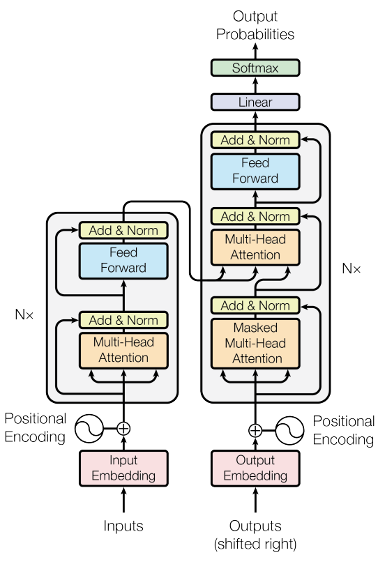
\includegraphics[scale=1.3]{gambar/TransformerArsitektur.png}
  \caption{Arsitektur Transformer}
  \label{fig:transformerArsitektur}
\end{figure}

Namun, meskipun kemajuan ini sangat mengesankan, NLP juga menghadapi beberapa tantangan besar. Salah satu tantangan utama adalah penanganan ambiguasi bahasa dan konteks yang sangat bergantung pada nuansa semantik. Model-model NLP harus dilatih dengan data yang cukup besar dan beragam untuk memahami konteks yang kompleks dan mengurangi bias. Masalah ini menjadi fokus penelitian untuk memastikan bahwa model-model NLP dapat menghasilkan hasil yang akurat dan adil~(\cite{brown2020}).

Di samping itu, aplikasi NLP dalam berbagai industri juga berkembang dengan cepat. Dalam layanan pelanggan, misalnya, \emph{chatbots} yang didukung oleh teknologi NLP dapat menangani permintaan pelanggan dengan lebih efisien dan menyediakan dukungan 24/7. Di sektor kesehatan, NLP digunakan untuk menganalisis catatan medis dan memberikan wawasan yang berguna untuk diagnosis dan perawatan. Perkembangan ini menunjukkan bagaimana NLP dapat mempengaruhi berbagai aspek kehidupan sehari-hari dan bisnis~(\cite{peters2018}).

\subsection{HuggingFace}

HuggingFace adalah sebuah perusahaan yang dikenal sebagai pemimpin
dalam bidang \emph{Natural Language Processing} (NLP). Misi inti mereka adalah 
membuat teknologi NLP yang kuat dan canggih lebih mudah diakses 
oleh para peneliti, ilmuwan data, pengembang, dan 
perusahaan~(\cite{huggingface}). Salah satu kontribusi 
utama HuggingFace adalah penyediaan berbagai model NLP 
\emph{"state-of-the-art"} yang telah dilatih dengan data 
besar, seperti model BERT, DistilBert, GPT-2, DistilGPT2, 
dan banyak lagi. Model-model ini sangat kuat dan dapat 
digunakan dalam berbagai tugas, seperti penerjemahan bahasa, 
analisis sentimen, generate teks otomatis, dan pemahaman 
bahasa alami~(\cite{wolf2020}). Selain itu, HuggingFace juga 
menyediakan API yang mempermudah penggunaan model NLP 
tersebut. Mereka juga mengembangkan alat-alat dan 
perpustakaan \emph{(library)} yang mendukung pengembangan 
dan penelitian di bidang NLP~(\cite{inference}). Dengan demikian, 
HuggingFace berperan penting dalam memperluas akses ke teknologi 
NLP canggih, memungkinkan inovasi di berbagai industri, termasuk 
pemrosesan teks, layanan pelanggan, penelitian akademik, dan 
banyak lagi~(\cite{azure}).

HuggingFace menyediakan platform yang sangat terintegrasi, seperti model hub dan datasets hub, yang memungkinkan pengguna untuk mengakses dan berbagi model serta dataset dengan mudah. Model hub, misalnya, adalah repositori online di mana pengguna dapat menemukan berbagai model pre-trained dari berbagai jenis dan domain, yang siap digunakan untuk berbagai aplikasi NLP. Ini mempercepat proses eksperimen dan pengembangan, memungkinkan peneliti dan pengembang untuk fokus pada pemecahan masalah dan aplikasi inovatif tanpa perlu memulai dari nol~(\cite{huggingface}).

Salah satu alat unggulan dari HuggingFace adalah Transformers library, yang menyediakan antarmuka intuitif untuk menggunakan model-model NLP canggih. Library ini mempermudah integrasi model dengan aplikasi yang ada dan menyediakan berbagai fungsionalitas, termasuk pelatihan ulang (fine-tuning) dan evaluasi model. Dengan dokumentasi yang lengkap dan komunitas aktif, Transformers library telah menjadi pilihan utama bagi banyak praktisi di bidang NLP untuk membangun dan menyebarluaskan aplikasi berbasis teks~(\cite{wolf2021}).

HuggingFace juga aktif dalam komunitas penelitian dengan mengadakan konferensi, workshop, dan publikasi penelitian terkait NLP. Mereka berfokus pada kolaborasi dengan akademisi dan industri untuk mendorong batasan-batasan teknologi NLP dan menghadirkan inovasi terbaru dalam model bahasa dan teknik pemrosesan bahasa alami. Dengan upaya ini, HuggingFace tidak hanya menyediakan alat dan sumber daya tetapi juga berkontribusi pada kemajuan ilmiah di bidang NLP~(\cite{huggingface}).



\subsection{DistilGPT2}

DistilGPT2 Model dipilih sebagai model yang akan digunakan pada 
penelitian ini. DistilGPT2 adalah model NLP yang dikembangkan oleh 
HuggingFace, yang merupakan versi ringan (distil) dari model 
\emph{GPT-2 (Generative Pre-trained Transformer 2)}. Keunggulan 
DistilGPT2 terletak pada efisiensi komputasi, membuatnya sangat 
cocok untuk aplikasi yang membutuhkan pemrosesan teks cepat dalam 
skala besar. DistilGPT2 mempertahankan arsitektur dasar GPT-2 dengan 
lapisan dan parameter lebih sedikit, membuatnya lebih ringan dan cepat. 
Meskipun lebih kecil, DistilGPT2 mampu menghasilkan teks dengan baik 
dan cocok untuk aplikasi NLP pada perangkat dengan sumber daya 
terbatas. Hasil evaluasi menunjukkan bahwa DistilGPT2 memiliki 
performa yang kompetitif dan efisien. Hal ini membuat DistilGPT2 
menjadi pilihan yang menarik dalam pengembangan aplikasi yang 
bergantung pada analisis teks dengan kecepatan dan efisiensi~(\cite{buzea2022}). 
Arsitektur DistilGPT2 dapat dilihat pada Gambar 
\ref{fig:distilgpt2Architecture}.

\begin{figure}[H]
  \centering
  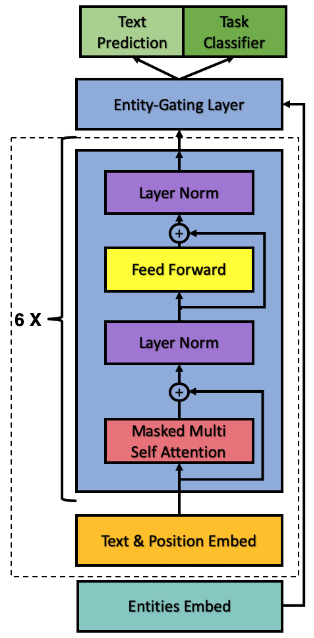
\includegraphics[scale=0.65]{gambar/DistilledGPT2Architecture.png}
  \caption{Arsitektur DistilGPT2}
  \label{fig:distilgpt2Architecture}
\end{figure}

Dalam pengembangan DistilGPT2, teknik distilasi pengetahuan digunakan untuk mengurangi ukuran model tanpa mengorbankan kualitas secara signifikan. Proses ini melibatkan pelatihan model kecil (DistilGPT2) untuk meniru output dari model besar (GPT-2). Dengan cara ini, model yang lebih kecil dapat belajar untuk menghasilkan teks dengan kualitas yang hampir sama dengan model yang lebih besar, namun dengan kebutuhan komputasi yang jauh lebih rendah~(\cite{sanh2019}).

Kelebihan lain dari DistilGPT2 adalah kemampuannya untuk melakukan inferensi dengan cepat, yang sangat penting dalam aplikasi real-time seperti chatbots dan sistem rekomendasi. Pengurangan ukuran model ini memungkinkan deployment pada perangkat dengan kapasitas memori dan daya komputasi yang terbatas, seperti smartphone dan perangkat IoT, tanpa mengorbankan kinerja~(\cite{merity2018}).

Selain efisiensi, DistilGPT2 juga menawarkan kompatibilitas yang tinggi dengan berbagai API dan framework NLP. Ini mempermudah integrasi dengan sistem yang sudah ada dan memungkinkan pengembang untuk memanfaatkan kekuatan model tanpa memerlukan konfigurasi yang kompleks. Library seperti Transformers dari HuggingFace menyediakan antarmuka yang intuitif untuk menggunakan DistilGPT2, memungkinkan implementasi yang lebih mudah dalam berbagai aplikasi~(\cite{wolf2020}).

Studi kasus penggunaan DistilGPT2 dalam berbagai aplikasi praktis menunjukkan bahwa model ini dapat menangani berbagai jenis teks dengan baik, dari analisis sentimen hingga pembuatan konten otomatis. Kecepatan dan efisiensinya membuatnya ideal untuk situasi di mana latensi rendah dan throughput tinggi adalah prioritas utama~(\cite{brown2020}).

Di masa depan, distilasi model seperti yang dilakukan dengan DistilGPT2 dapat menjadi metode standar untuk mengembangkan model NLP yang lebih efisien, seiring dengan kebutuhan yang terus berkembang untuk solusi yang hemat biaya dan cepat. Penelitian lebih lanjut dalam bidang ini diharapkan dapat mengoptimalkan teknik distilasi lebih lanjut dan memperkenalkan model-model yang lebih canggih dengan performa yang sebanding atau lebih baik~(\cite{clark2020}).

\subsection{FastAPI}

Untuk dapat menghubungkan antara DistilGPT2 Model dan program DISC 
yang menggunakan Titian, penelitian ini akan memanfaatkan FastAPI. 
FastAPI adalah kerangka kerja web Python yang dikenal dengan kinerja 
tinggi, kemudahan pengembangan, dan otomatisasi pembuatan dokumentasi 
API. Dibangun di atas Python 3.6+ yang mendukung asynchronous 
programming, FastAPI dapat menangani banyak permintaan dengan 
cepat. Kerangka kerja ini menggunakan teknologi seperti 
\emph{Starlette} dan \emph{Pydantic} untuk memastikan 
penanganan permintaan HTTP yang efisien dan validasi data 
yang kuat~(\cite{fastapi}). Hingga kini FastAPI telah banyak 
dimanfaatkan untuk keperluan machine learning dan data science 
dan terbukti 45\% jauh lebih baik dibandingkan dengan 
Flask~(\cite{bansal2022}). Flask adalah framework web Python 
yang ringan dan fleksibel yang menekankan kesederhanaan dan 
kemampuan untuk diperluas. Ini menyediakan fitur dasar untuk 
pengembangan web dan memungkinkan pengembang memilih dan 
mengintegrasikan ekstensi berdasarkan kebutuhan 
proyek mereka~(\cite{kotha2023}).

FastAPI menawarkan kelebihan signifikan dalam hal kecepatan dan efisiensi dibandingkan dengan kerangka kerja web lainnya. Salah satu fitur utama dari FastAPI adalah kemampuannya untuk menghasilkan dokumentasi API secara otomatis menggunakan OpenAPI dan JSON Schema. Dokumentasi ini sangat berguna untuk pengembang dalam memahami dan mengintegrasikan API dengan lebih mudah. FastAPI juga memanfaatkan fitur typing dari Python untuk melakukan validasi dan konversi data secara otomatis, mengurangi kemungkinan kesalahan dan meningkatkan keandalan aplikasi~(\cite{fastapi}).

Dalam konteks machine learning, FastAPI memfasilitasi pembuatan dan penyebaran model dengan lebih efisien. Misalnya, saat menghubungkan model DistilGPT2 dengan aplikasi DISC, FastAPI memungkinkan integrasi model ke dalam endpoint API yang dapat diakses dengan mudah oleh aplikasi lain. Hal ini memungkinkan komunikasi yang cepat antara model dan aplikasi, serta memungkinkan pemrosesan data yang lebih efisien. FastAPI mendukung berbagai format data seperti JSON, yang umum digunakan dalam interaksi dengan model machine learning~(\cite{ariful2021}).

Keamanan juga merupakan fitur penting dari FastAPI. Kerangka kerja ini menyediakan berbagai mekanisme untuk melindungi aplikasi dari serangan umum, seperti injeksi SQL dan serangan XSS (cross-site scripting). FastAPI mendukung berbagai metode autentikasi dan otorisasi, termasuk OAuth2 dan JWT, yang memastikan bahwa hanya pengguna yang terverifikasi yang dapat mengakses endpoint API tertentu. Dengan fitur-fitur ini, FastAPI membantu dalam membangun aplikasi yang aman dan terkelola dengan baik~(\cite{bansal2022}).

FastAPI telah terbukti efektif dalam skenario produksi, dengan berbagai studi kasus yang menunjukkan kemampuannya untuk menangani beban tinggi dan volume permintaan yang besar dengan kinerja yang stabil. Dengan dukungan komunitas yang aktif dan terus berkembang, serta integrasi yang mudah dengan berbagai alat dan teknologi modern, FastAPI semakin menjadi pilihan populer untuk pengembangan API yang cepat dan efisien~(\cite{fastapi}).

\subsection{Uvicorn}

Uvicorn adalah server web asinkron yang berbasis di Python.
Uvicorn dirancang untuk menangani permintaan HTTP secara
asinkron, yang memungkinkan server untuk menangani banyak
permintaan secara bersamaan tanpa memblokir proses. Uvicorn
menggunakan teknologi seperti \emph{ASGI (Asynchronous Server
Gateway Interface)} dan \emph{asyncio} untuk memastikan
penanganan permintaan HTTP yang efisien dan cepat. Uvicorn
juga mendukung fitur-fitur seperti \emph{websockets} dan
\emph{server push}, yang memungkinkan pengembang untuk
membangun aplikasi web yang interaktif dan responsif.
Dengan kinerja yang cepat dan kemampuan asinkronnya, Uvicorn
cocok digunakan dalam aplikasi web yang membutuhkan
penanganan permintaan HTTP yang cepat dan efisien~(\cite{uvicorn}).

Salah satu keuntungan utama menggunakan Uvicorn adalah kemampuannya untuk mengelola beban kerja yang tinggi dengan latensi rendah. Karena mendukung asynchronous I/O, Uvicorn dapat melayani banyak permintaan secara bersamaan tanpa perlu membuat thread baru untuk setiap permintaan. Ini mengurangi overhead dan meningkatkan throughput server secara keseluruhan, membuatnya ideal untuk aplikasi yang memiliki volume lalu lintas tinggi~(\cite{skjerven2022}).

Uvicorn juga terkenal karena kemudahan penggunaannya dan integrasinya dengan berbagai framework Python modern. Ketika digunakan bersama dengan FastAPI, misalnya, Uvicorn dapat secara otomatis menangani routing, validasi, dan dokumentasi API, memungkinkan pengembang untuk fokus pada logika aplikasi. Integrasi ini mempermudah proses pengembangan dan deployment aplikasi web, serta meningkatkan produktivitas pengembang~(\cite{hwang2021}).

Dalam hal keamanan, Uvicorn menyediakan berbagai fitur untuk melindungi aplikasi dari potensi ancaman. Misalnya, Uvicorn dapat dikonfigurasi untuk menggunakan TLS (Transport Layer Security) untuk enkripsi komunikasi data, serta mengimplementasikan header keamanan yang mencegah serangan umum seperti Cross-Site Scripting (XSS) dan Cross-Site Request Forgery (CSRF). Fitur-fitur ini membantu menjaga integritas dan kerahasiaan data yang ditransmisikan antara server dan klien~(\cite{nguyen2022}).

Uvicorn terus mendapatkan dukungan aktif dari komunitas dan pengembang, dengan pembaruan rutin yang memperkenalkan fitur-fitur baru dan perbaikan keamanan. Dokumentasi yang komprehensif dan komunitas yang aktif memudahkan pengembang untuk memanfaatkan fitur-fitur terbaru dan mendapatkan bantuan jika diperlukan. Dengan kinerja yang solid dan dukungan yang kuat, Uvicorn merupakan pilihan server web yang handal untuk aplikasi-asinkron modern~(\cite{smith2023}). 

\subsection{AWS EC2}

DistilGPT2 Model yang ditanamkan ke dalam FastAPI kemudian 
akan di-\emph{deploy} menggunakan Amazon Web Service (AWS) EC2. 
AWS adalah platform komputasi awan yang dikelola oleh Amazon. 
AWS menyediakan berbagai layanan komputasi, penyimpanan, database, 
jari-ngan, dan lainnya yang dapat digunakan oleh perusahaan dan 
pengembang untuk menjalankan aplikasi mereka di lingkungan awan. 
Amazon EC2 adalah salah satu layanan inti di AWS yang memungkinkan 
pengguna untuk menyewa mesin virtual \emph{(instance)} di \emph{cloud}. 
Pengguna dapat memilih berbagai jenis instance yang sesuai dengan 
kebutuhan mereka, seperti instance berkinerja tinggi, \emph{instance} 
berbasis GPU, atau \emph{instance} berbiaya rendah. AWS EC2 
memungkinkan pengguna untuk dengan cepat meluncurkan, mengelola, 
dan menghentikan instance sesuai kebutuhan, sehingga mereka dapat 
mengskalakan aplikasi mereka sesuai dengan permintaan dan menghemat 
biaya saat instance tidak digunakan~(\cite{vohra2016}). Dibandingkan 
dengan kompetitornya, AWS EC2 menawarkan solusi yang lebih baik di 
mana pengguna dapat memiliki kesempatan untuk memilih fitur yang 
diinginkan sesuai kebutuhan~(\cite{kumar2021}).

Salah satu kelebihan utama AWS EC2 adalah kemampuannya untuk menawarkan berbagai jenis instance yang disesuaikan dengan berbagai kebutuhan komputasi. Misalnya, instance berbasis GPU seperti seri P dan G dirancang khusus untuk aplikasi yang memerlukan pemrosesan grafis berat, seperti pelatihan model machine learning. Sebaliknya, instance tipe T dan M cocok untuk aplikasi dengan kebutuhan komputasi umum dan memberikan keseimbangan antara CPU, memori, dan biaya~(\cite{aws2022}).

AWS EC2 juga menyediakan fitur keamanan yang canggih untuk melindungi data dan aplikasi. Pengguna dapat memanfaatkan Amazon Virtual Private Cloud (VPC) untuk mengisolasi lingkungan jaringan mereka, serta menggunakan security groups dan network access control lists (ACLs) untuk mengontrol akses ke instance mereka. Selain itu, AWS EC2 mendukung enkripsi data baik dalam transit maupun saat disimpan, memastikan bahwa data sensitif dilindungi dari potensi ancaman~(\cite{sharma2021}).

Fitur auto-scaling di AWS EC2 memungkinkan pengguna untuk secara otomatis menambah atau mengurangi jumlah instance berdasarkan permintaan aplikasi. Ini sangat berguna untuk menangani lonjakan lalu lintas atau beban kerja yang bervariasi tanpa memerlukan intervensi manual. Auto-scaling membantu menjaga performa aplikasi tetap optimal sambil meminimalkan biaya operasional dengan hanya menjalankan instance yang diperlukan pada waktu tertentu~(\cite{tang2021}).

Terakhir, AWS EC2 menawarkan integrasi yang mulus dengan berbagai layanan AWS lainnya, seperti Amazon RDS untuk database, Amazon S3 untuk penyimpanan objek, dan AWS Lambda untuk menjalankan kode tanpa server. Integrasi ini memungkinkan pengembang untuk membangun solusi yang terintegrasi dan skalabel dengan memanfaatkan ekosistem layanan yang luas dan kuat dari AWS~(\cite{chen2023}). 
Arsitektur AWS EC2 dan fitur-fiturnya dapat dilihat 
pada gambar \ref{fig:awsEC2Architecture}.

\begin{figure}[H]
  \centering
  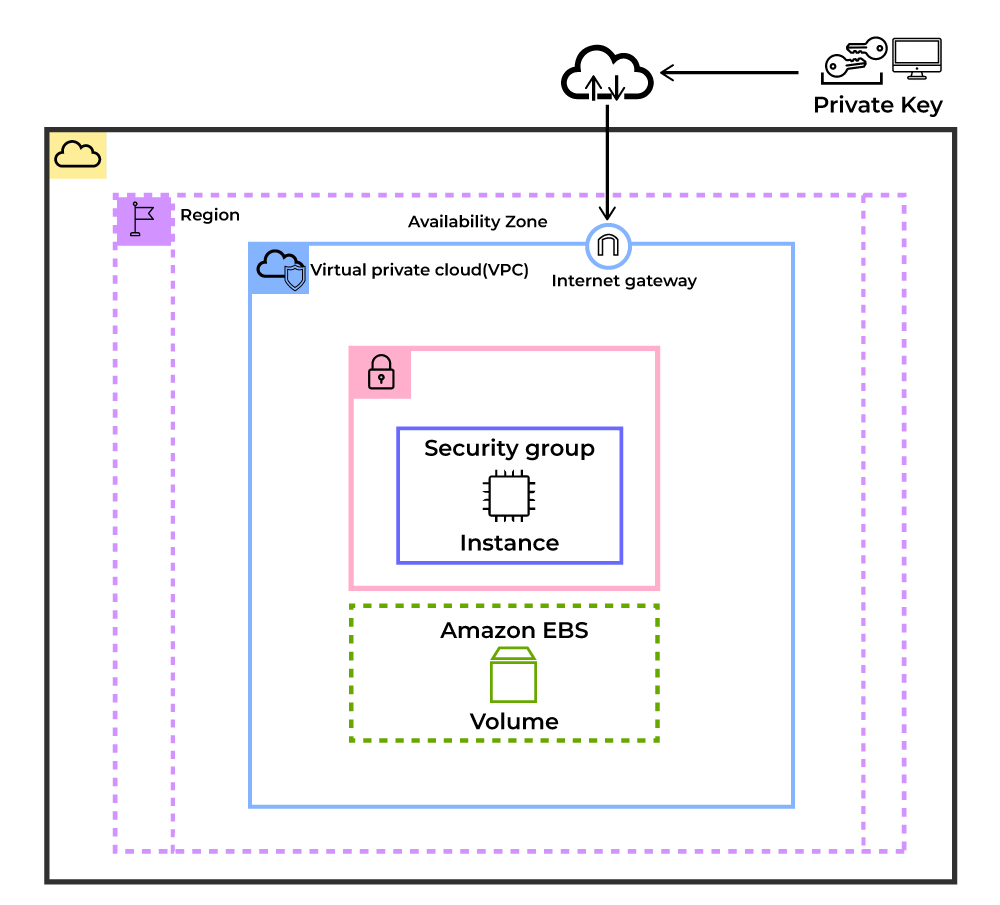
\includegraphics[scale=0.4]{gambar/ec2arsitektur.png}
  \caption{Arsitektur AWS EC2~(\cite{geeksforgeeks})}
  \label{fig:awsEC2Architecture}
\end{figure}


\subsection{Python Programming Language}
Python adalah bahasa pemrograman tingkat tinggi yang sering
digunakan dalam pengembangan aplikasi web, ilmu data, dan
kecerdasan buatan. Python memiliki sintaksis yang sederhana
dan mudah dipahami, sehingga sangat cocok untuk pemula dan
pengembang yang tidak memiliki latar belakang pemrograman
yang kuat. Python juga memiliki ekosistem yang kaya, dengan
ribuan \emph{library} dan \emph{framework} yang mendukung
pengembangan aplikasi web, ilmu data, dan kecerdasan buatan.
Pada proses training awal model dan pembuatan FastAPI, bahasa 
pemrograman yang akan digunakan adalah Python. Python dipilih 
untuk proses training awal model dan pembuatan FastAPI karena 
memiliki sintaksis yang mudah dipahami, ekosistem yang kaya, 
serta banyak \emph{library} dan \emph{framework} yang 
mendukung pengembangan aplikasi \emph{machine learning} dan 
web termasuk HuggingFace. Kelebihan Python dalam kesederhanaan 
dan kemudahan penggunaan membuatnya menjadi pilihan utama dalam 
fase awal pengembangan~(\cite{sharma2020}).

\section{Scala Programming Language}
Pada proses penanaman Titian, pembuatan sistem yang akan 
mengonsumsi FastAPI, dan pengujian sistem,
bahasa pemrograman yang akan digunakan adalah Scala. 
Scala adalah bahasa pemrograman yang berjalan di atas
\emph{Java Virtual Machine} (JVM) dan dirancang untuk menyatukan
keuntungan dari bahasa pemrograman fungsional dan objek.
Scala dipilih untuk pembuatan sistem yang mengonsumsi FastAPI 
karena Scala menawarkan keunggulan dalam hal konkurensi dan 
eksekusi paralel, yang dapat meningkatkan kinerja sistem secara 
signifikan. Pemilihan Scala juga didorong oleh keandalan dan 
ekosistem yang mapan, terutama dalam pengembangan aplikasi 
berukuran besar~(\cite{laddad2020}). Dibandingkan dengan Java 
pada bidang \emph{Natural Language Processing (NLP)}, Scala 
dianggap lebih unggul karena ekosistemnya yang lebih modern 
dan fitur-fitur fungsional yang dapat mempermudah pengembangan 
aplikasi NLP~(\cite{pankratius2012}). Scala memungkinkan 
penggunaan paradigma fungsional yang mendukung pemrosesan 
data kompleks dan manipulasi struktur data dengan lebih 
efisien, sehingga menjadi pilihan yang tepat untuk tugas-tugas 
kompleks dalam NLP~(\cite{papadimitriou2011}).